%!TEX program = xelatex
% !BIB program = bibtex
\documentclass[12pt,letterpaper]{article}
\usepackage{./style/dsc180reportstyle} % import dsc180reportstyle.sty

%%%%%%%%%%%%%%%%%%%%%%%%%%%%%%%%%%%%%%%%%%%%%%%%%%%%%%%%
%%%% Title and Authors
%%%%%%%%%%%%%%%%%%%%%%%%%%%%%%%%%%%%%%%%%%%%%%%%%%%%%%%%

\title{Privacy in Practice: The Feasibility of Differential Privacy for Telemetry Analysis}

\author{Trey Scheid \\
  {\tt tscheid@ucsd.edu} \\\And
  Tyler Kurpanek \\
  {\tt tkurpane@ucsd.edu} \\\And
  Bradley Nathanson \\
  {\tt bnathanson@ucsd.edu} \\\And
  Christopher Lum \\
  {\tt cslum@ucsd.edu} \\\And
  Yu-Xiang Wang \\
  {\tt yuxiangw@ucsd.edu} \\}

\begin{document}
% INSERT TITLE
% title is defined above
\maketitle



%%%%%%%%%%%%%%%%%%%%%%%%%%%%%%%%%%%%%%%%%%%%%%%%%%%%%%%%
%%%% Abstract and Links
%%%%%%%%%%%%%%%%%%%%%%%%%%%%%%%%%%%%%%%%%%%%%%%%%%%%%%%%

\begin{abstract}    
  This research investigates the implementation implications of differential privacy mechanisms for telemetry data analysis, with a focus on real-world applications. We show, through examples, how knowledge of fundamental privacy-preserving techniques, including randomized response and the Laplace mechanism, is enough to protect sensitive information while maintaining analytical utility. We privatize data tasks from 4 applied research works using Intel telemetry data which   encompasses multiple statistical tasks, from user-level rate analysis to logistic regression classification. The study utilizes various $(\epsilon, \delta)$ budgets (using AutoDP) for precise privacy loss measurement and to quantify the inherent tradeoff between privacy and utility. By demonstrating the feasibility of differential privacy in production environments, we provide a roadmap for organizations seeking to enhance their privacy practices.
  \begin{center}
    Website: \url{https://trey-scheid.github.io/privacy-in-practice/} \\
    Code: \url{https://github.com/Trey-Scheid/privacy-in-practice}
  \end{center}
\end{abstract}

\clearpage

% TABLE OF CONTENTS
{\Large\bf\raggedright Table of Contents}

\maketoc

\clearpage

%%%%%%%%%%%%%%%%%%%
%%%% INTRO %%%%%%%%%%%
%%%%%%%%%%%%%%%%%%%

\section{Introduction}

The implementation of differential privacy in production environments presents significant challenges in balancing privacy guarantees with analytical utility. This research addresses these challenges by developing practical privacy-preserving mechanisms for existing telemetry analysis tasks while maintaining the usefulness of their systems. We integrate various differential privacy mechanisms including: Gaussian Composition, the Exponential\/Laplace mechanism, and \_\_ to protect sensitive information in telemetry data. Our chosen data tasks encompasses multiple statistical tasks, from user-level rate analysis to logistic regression classification correlation. By evaluating the trade-offs between privacy guarantees and analytical accuracy in production settings, we provide evidence and direction for organizations looking to enhance their privacy practices.

\subsection{Motivation}

Despite the growing importance of privacy-preserving data analysis \cite{PewPrivacy2019}, many practitioners perceive differential privacy implementation as complex and challenging, others note how results only come with dissatisfactory $\epsilon$-level guarantees \cite{FLandPrivacy}. Besides the sub-optimality of some DP methods, this perception stems from human difficulties: the mathematical complexity of privacy definitions, the need to carefully calibrate privacy parameters, and concerns about reduced utility (managing the trade-off) \cite{DP-fyML}. A survey by Smith et al. found that only 23\% of data scientists felt confident implementing differential privacy mechanisms in their workflows \cite{needed3}. Researchers are working to democratize, demystify, and improve usability around Differential Privacy \cite{DP-fyML}. Recent developments have significantly lowered these barriers to entry. Tools like Google's Privacy on Beam \footnote{\url{https://codelabs.developers.google.com/codelabs/privacy-on-beam}}, Microsoft's SmartNoise \footnote{\url{https://smartnoise.org}}, and various open-source libraries like AutoDP\footnote{\url{https://pypi.org/project/autodp/}} provide accessible frameworks for implementing differential privacy. These tools abstract away much of the underlying complexity while maintaining rigorous privacy guarantees. In addition, educational resources and practical tutorials have emerged to guide practitioners through implementation challenges \footnote{\url{https://desfontain.es/blog/friendly-intro-to-differential-privacy.html}}.

%"has been observed that limiting sensitivity even with small amounts of noise (or no noise at all) can significantly reduce memorization.18 This gap is to be expected, as DP assumes a “worst-case adversary’’ with infinite computation and access to arbitrary side information. These assumptions are often unrealistic in practice. Thus, there are substantial advantages to training using a DP algorithm that limits each user’s influence, even if the explicit random noise introduced into the training process is not enough to ensure a small ε formally. Nevertheless, designing practical FL and FA algorithms that achieve small ε guarantees is an important area of ongoing research."

This research builds upon these recent developments by providing a practical demonstration of differential privacy mechanisms in telemetry data analysis. By implementing privacy-preserving techniques for existing tasks, we aim to show that differential privacy can be seamlessly integrated into production systems without significant utility loss. Our work focuses on two key objectives: privatizing existing telemetry analysis tasks and evaluating the privacy-utility tradeoffs in production settings.

\subsection{Differential Privacy}

Differential privacy by \cite{DworkRoth} is a framework for data privacy that gives a mathematical guarantee that the information for each individual (record or user) in the dataset is protected\footnote{\cite{DP-def} has an in depth explanation of interpretations and attacks.}. The core idea is to introduce random noise into algorithms so that the data of any individual does not significantly affect the overall result and therefore is not recoverable or identifiable. 

Mathematically, a mechanism $M$ is considered $(\epsilon, \delta)$ differentially private if for all datasets $D$ and $D'$ which differ by at most 1 element when $\P [ M(D)\in S ] \leq e^\epsilon \P [ M(D') \in S)] + \delta$ where $\epsilon$ and $\delta$ are privacy parameters and $S$ is a query solution set. Smaller $\epsilon$ and $\delta$ imply stronger privacy guarantees. Differential privacy is a \textit{property} of algorithms, not datasets; it is a method that ensures private results to a high degree of probability (whether that is a trained model or a noisy dataset). 

This definition applies to data anonymization, but does not cover methods for transparency, use, access or security. By pursuing this property for common data tasks we aim to create a solution which once implemented achieves similar results but removes the need for data access and security. Some settings the predictions themselves are important, but sensitive, meaning a mechanism without anonymity is unusable!

\subsection{Telemetry Data}

The Intel Data Collection and Analysis (DCA) team derives insights from over 39 million systems! This includes any of their hardware installed in personal, corporate and IoT devices (collected only with consent). Through their partnership with the University of California San Diego's Halicioğlu Data Science Institute, at the foundation of Intel Lab's Telemetry Center of Excellence, they permit study of possibly sensitive device information to develop solutions that benefit the whole ecosystem \footnote{\url{https://community.intel.com/t5/Blogs/Tech-Innovation/Data-Center/Intel-Labs-Investment-in-Telemetry-Center-of-Excellence-Produces/post/1460669}}. Faculty and Intel researchers have published many white papers using the database since the CoE inception in 2020. We selected 4 of interest and found their core data science methods Table \ref{tab:DataTasks}.

\begin{table}[h]%!
\begin{center}
\caption{Data Tasks}
\label{tab:DataTasks}
\begin{tabular}{|p{4.5cm}|p{2.5cm}|p{5cm}|p{2.7cm}|}
\hline
Data Task & Code & Paper & Citation \\
\hline
Conditional Probabilities & COND\_PROB & Exploration of CPU Error Dependencies and Prediction & \cite{Kwasnick2023} \\
\hline
KMeans Clustering & KMEANS & PC Health Impact White Paper & \cite{kmeans} \\
\hline
Lasso Regression & LASSO & Power Consumption Patterns in Intel’s Telemetry Data: China Burns 2x Energy that of the US & \cite{lassocarbon} \\
\hline
Logistic Regression Significance Tests & LR\_PVAL & Product Health Insights Using Telemetry & \cite{prodhealLR} \\
\hline
\end{tabular}
\end{center}
\end{table}

Differential privacy methods and guarantees are attractive for many domains. Telemetry is the remote data transfer of automated system measurements. As people use technology everyday their machines track usage diagnostics which are used by hardware and software manufacturers to reduce bugs and increase efficiency. System usage information is recorded at regular intervals and usually results in massive quantities of measurements. The identifiability of the specific machine or user of an event is a concern regardless of PIID tags. Dinur Nissim Reconstruction and linkage attacks can be used to recover or reconstruct the original information: the source \cite{DinurReconstruction}. This is a breach of privacy for a user which depending on the sensitivity of the information can be concerning. For example, personal laptops may send diagnostics to Intel given that the user opts in to the program [Intel telemetry]. 

We use a secure research database shared be Intel Corporation with consent of its users to generate real results....

\subsubsection{Errors}

In our paper, we will analyze two different types of errors. The Machine Check Architecture, or MCA, will detect an error and label it as either corrected or uncorrected. A corrected error means the system can observe and correct a detected error. Correction mechanisms include single error correction, double error correction, and more. An uncorrected error is one that was detected but not corrected or there was a computation delay long enough that the MCA treated it as an interrupted computation. \cite{Kwasnick2023}

\subsubsection{Hardware Power [not done yet]}

Another concept is power, this is the rate of energy consumption by the device. Our analysis is on CPU's produced by Intel and AMD. \cite{Kwasnick2023}

\subsection{Applications [not done yet]}

Telemetry is one narrow domain which privacy is a concern, many other types of data require sensitive handling and sharing practices. For example the US Census \footnote{need citation}. 

We will get into the specifics of each task, however note that each one can be applied to datasets about any interest. probabilities of political party affiliation, Lasso/kmeans for gene identification, or correlation for \_\_. 

\subsection{Related Work}

We are building on a previous analysis on differentially private mechanisms for Logistic Regression  \cite{qtr1proj}. The paper investigates how privacy affects different mini-batch stochastic gradient descent algorithms for logistic regression classification. It is shown that privacy affects the batch size for optimal performance.

%%%%%%%%%%%%%%%%%%%
%%%%  METHODS  %%%%%%%%
%%%%%%%%%%%%%%%%%%%

\section{Methods}

\subsection{Utility}

Each method used in our study has different measures of success, but they can all be translated into a proportion representing utility compared to the best model, whether that is the non-private baseline or an improved version. In the context of differential privacy, utility refers to the degree to which a privatized model or analysis retains its analytical accuracy and usefulness compared to its non-private counterpart.


\subsection{Data Structure}

The first sub-task was data ingestion and processing. One key feature of telemetry data is the volume; the research database was already a processed version of raw signals from devices, aggregated and merged for usefulness and practicality. This left us with a schema containing 10's of tables and cryptic metrics, highlighting the importance of documentation by our fellow researchers to help us replicate their work.

The tables once loaded to disc could be processed with SQL queries and filtered and processed with more basic operations such as aggregating by group and finding statistics. These would make up our featurized datasets ready for Python analysis.

\subsection{LR\_PVAL: Private Correlation (via Logistic Regression Coefficient)}

This paper\footnote{needs citation} seeks to identify whether a certain variable is disproportionately present for a certain outcome. 
More specifically, it takes a close look at two variables, max temperature on a day and whether a corrected error was present on that day. 
They would take one of those two variables and train a logistic regression model with maximum likelihood estimation to predict whether an uncorrected error was present.
From the model, they use the coefficient of the variable and make a hypothesis test whether that variable is equal to zero.

For our implementation, we focused only on whether there were corrected errors on a day, and not the variable max temperature on a day.
We add privacy to the model by using DP-SGD when training the logistic regression model, where the hypothesis test is then private by means of post-processing.
We replicated the non-private model to get a baseline for utility and compared it to our private model using set intersection over union.
Our data came from Intel's telemetry database, which contains information about the hardware and software on millions of devices
and we took a subset of one year of the data from Februrary 2020 to 2021.

\subsubsection{Nonprivate Logistic Regression}

The paper used a univariate logistic regression model, one for each of the top 30 uncorrected error codes.
The target variable is whether or not an uncorrected error was present on a day, 
and the feature a boolean of whether there was a corrected error on that day, 
making uncorrected error ~ corrected error.

The logistic regression model is defined as 

\begin{equation}
    \label{eq:logistic_regression}
    \log \frac{P(y=1|x)}{1-P(y=1|x)} = \beta_0 + \beta_1 x
\end{equation}

and they took $\beta_1$ as the coefficient of interest.
They used a Wald test to test the null hypothesis that $\beta_1 = 0$ against the alternative that $\beta_1 \neq 0$.
The Wald test statistic is defined as 

\begin{equation}
    \label{eq:wald_test}
    W = \frac{\hat{\beta}_1}{SE(\hat{\beta}_1)}
\end{equation}

where $\hat{\beta}_1$ is the coefficient estimate and $SE(\hat{\beta}_1)$ is the standard error of the coefficient estimate.
This statistic can be used to test whether or not the feature is significant in predicting the target variable (whether the presence of a corrected error is associated with the presence of an uncorrected error).
For our implementation, we used the statsmodels library to fit the model and calculate the coefficient and standard error with an alpha of 0.05.

\subsubsection{Private Logistic Regression}

In order to add privacy to the model, we used DP-Gradient Descent to train the model.
DP-GD is a method of training a model with differential privacy by adding noise to the gradient updates using Gaussian noise.
Each iteration of gradient descent adds a little bit more noise, consuming a proportion of the privacy budget, 
meaning that higher epsilons require more iterations.
We considered using DP-Stochastic Gradient Descent, but the processed datasets were small enough to warrant using DP-GD.
We implemented our own DP-GD algorithm using AutoDP\footnote{\url{https://pypi.org/project/autodp/}} to account for our privacy budget.
After privately training the model, post-processing enabled us to calculate the wald test the same way as in the non-private model.
In order to compare the alpha values, we completed permutation testing on each model in order to calculate the empirical p-value which was used to identify models that were statistically significant.
One of the thirty models had exceptionally more values than the others, so to save compute we removed it from the analysis.

\subsubsection{Utility}

We defined our utility metric as the set intersection over union of the top 29 uncorrected error codes.
This metric has a range of 0 to 1, where 0 is no intersection and 1 is full intersection,
meaning that the higher the utility, the more similar the two results are.

\subsection{LASSO Private Regression (via DP-Frank-Wolfe)}

will add lots of detail about lasso, then talk about adapting franke-wolfe to be differentially private. 

% Since the model is predicting power\_mean [SUM(pw.nrs * pw.mean) / SUM(pw.nrs)] which is a weighted average of some power rate metric in Watts I did some research. I found that 50W is a normal CPU and they typically range 10-150W with GPU up to 500-1000W which aligns with some EDA.

% Therefore, the features and coefficients found by LASSO represent the main culprits for energy consumption across all Intel devices which gets straight at the goal of the paper to reduce emissions! 

% 2. How can I interpret whether 5 or 50 or 500 mse watts is a reliable model? I found a model that predicts the average for each column gets around 40 mse watts. 

% 3. Also if power\_mean is in watts, would mse be watts^2 and root mse be watts, so we should report root mse?

% The interpretation of RMSE depends on the context. This requires us to think about how big of a difference is 3/30/300 watts for CPU power consumption?

% i.e., if MSE ≈ 15, we have RMSE ≈ 3.87. I would say a difference of 4 watts is not that bad.

\subsubsection{Utility}

\subsection{KMEANS Private Clustering (DP-Lloyd's)}
K-Means clustering (Lloyd's Algorithm) is applied to group devices based on similarities in their usage patterns. The method leverages Z-scores for standardizing the usage data and calculates L1 distances between weekly usage patterns to identify trends over time. Lloyd's Algorithm clusters devices by assigning them to centroids based on their usage patterns, recalculating the centroids as the mean of assigned points after each iteration. 

Differentially Private Lloyd's Algorithm (DP-Lloyd's)\footnote{\url{https://arxiv.org/pdf/1504.05998}} modifies the standard K-Means clustering by adding Laplacian noise during the iterative centroid update step to ensure privacy. It introduces noise to both the sum of coordinates and the count of points within clusters, with the amount of noise controlled by the number of iterations and the sensitivity of the data. This is applied after clipping the data, to for ensure that the impact of any single data point is limited. 
\[
\text{x'}_j = \text{clip}\left( \text{x}_j, -\tau, \tau \right)
\]

After clipping the data, the sum of each cluster is computed with added Laplace noise. \\One point changes the sum, at most, the range of the dataset, which is $2 \times \tau$ (the sensitivty). The number of data points is at least 1 if the cluster exists, and so one data point changes the count by 1. The sensitivity is therefore 1. These sensitivities are then divided by the per-iteration  \epsilon.

\[
\text{new\_centroid}_j=
\frac{
    \sum_{i=1}^{n_j} \text{x'}_{j,i} + \text{Lap}(\tau \times 2, \epsilon_{\text{iter}})
}{
    \max\left( 1, n_j + \text{Lap}(1, \epsilon_{\text{iter}}) \right)
}
\]

\subsubsection{Utility}
To calculate the utility for the K-Means task, we defined the loss for each
epsilon as the sum of squared distances between each data point and its closest centroid. We then divided it by the number of data point so it is agnostic to the dataset size. We then normalized the loss so that each loss value fell between 0 and 1 and defined the utility as
1-loss to inverse it.



\subsection{COND\_PROB: Private Conditional Probability Release (Laplace Mechanism)}
In order to replicate the paper, were are going to apply differential privacy methods to the processes outlined in the paper. In the paper, the authors first separate each GUID (user) into the number of corrected errors observed during a set time period. They then created a histogram where the x-axis was the number of corrected errors observed and the y-axis was the percentage of GUID's that observed an uncorrected error.\cite{Kwasnick2023} This is the process that we are aiming to privatize. 

We are releasing a percentage for each bin in the histogram, and in order to guarantee privacy, we must add noise to to both the numerator and denominator where the numerator is the number of GUID's that contained an uncorrected error (number of 1's) and the denominator is the number of GUID's total. However we can not release the number of GUID's in each corrected error count as that would violate differential privacy so instead we are just going to add noise to number of GUID's that contained an uncorrected error as well as the number of GUID's that did not contain an uncorrected an error (number of 1's + number of 0's) so that we have a private denominator. 

\[
P(Uncorrected) = \frac{\text{GUID's containing an Uncorrected Error}}{\text{Total GUID's}}
\]

We are going to apply the Laplace mechanism to to release this percentage privately. The Laplace mechanism adds noise drawn from the Laplace distribution to the output of a function. B is the scale parameter and $\nabla f$ is the sensitivity of the function f. \cite{DworkRoth}


$$noise \sim Lap(b) $$
$$Lap(x|b) = \frac{1}{2b}e^{-\frac{|x|}{b}}$$
$$b = \frac{\Delta f}{\epsilon}$$

The sensitivity of the function is defined as the maximum possible absolute change in the output of the function due to the change in a single user's data. Since we are dealing with a percentage (and we are considering the worst case), this change can be at most 1 user, which corresponds to a sensitivity of 1 (in terms of the scale of the count, not the percentage itself). This is because, in the worst case, the change is a single user being added or removed, and the total number of GUIDs is assumed to be large enough that the effect of one user's change on the output is not too significant.and $\nabla f$ is the privacy parameter. 
\begin{center}
$$\Delta f = \max_{D, D'} ||f(x) - f(x')|| = 1$$ \\
\text{D and D' are neighboring datasets}
\end{center}

\subsubsection{Utility}

To calculate the utility for the Conditional Probability task, we defined the loss for each epsilon as the Mean Absolute error between the Noisy and Original Histograms. We then normalized the loss so that each loss value fell between 0 and 1 and defined the utility as 1/loss. 







%%%%%%%%%%%%%%%%%%%
%%%% RESULTS  %%%%%%%%%
%%%%%%%%%%%%%%%%%%%

\section{Results}

\subsection{All Tasks: Privacy vs Utility}

INSERT COMBINED PLOT

\subsection{COND\_PROB}

\begin{figure}[h!]
    \centering
    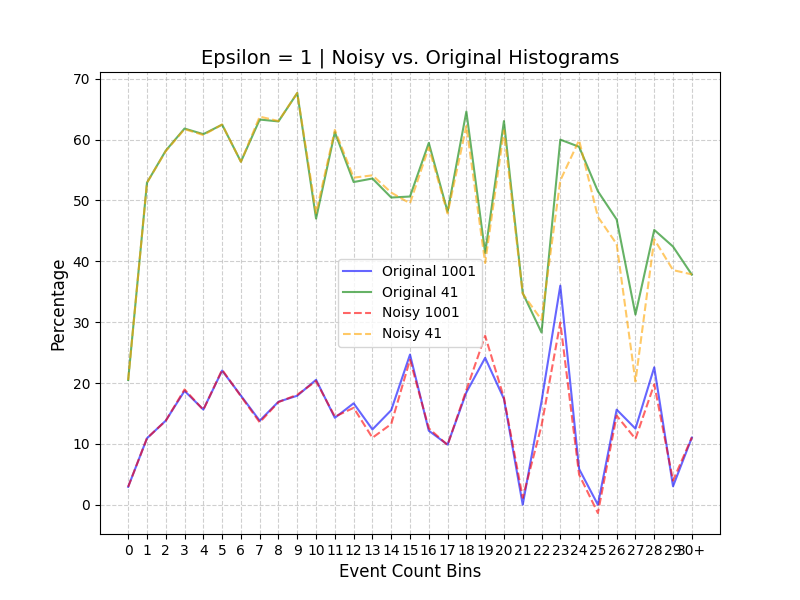
\includegraphics[width=0.8\textwidth]{report/figure/histoeps1.png}
    \caption{Your plot caption here.}
    \label{fig:yourplot}
\end{figure}



\subsection{LR\_PVAL}
\subsection{KMEANS}
\begin{figure}[H] % 'h' specifies to place the figure here in the text
    \centering
    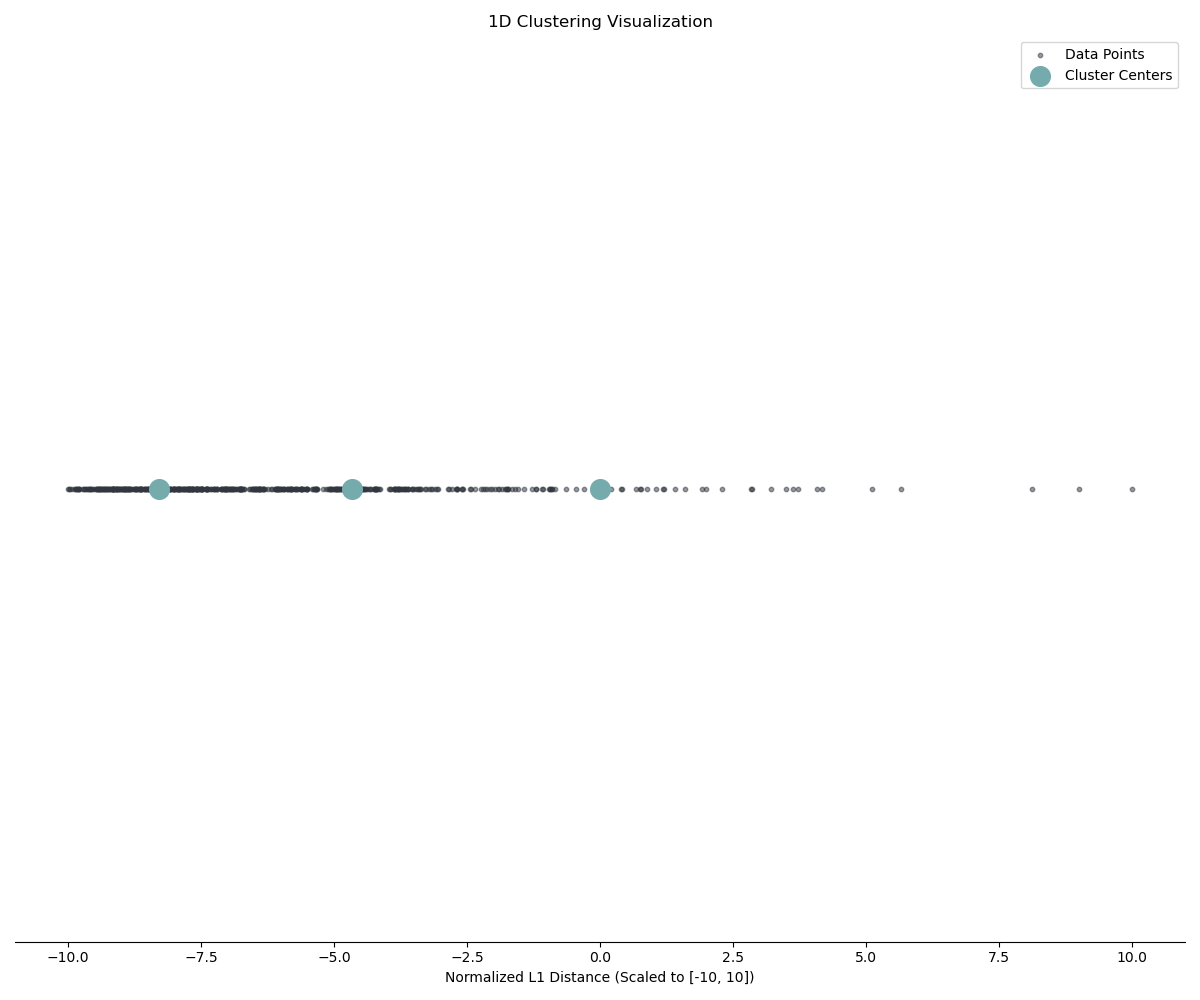
\includegraphics[width=0.6\textwidth]{figure/1d_clusters.png} % Path to the image
    \caption{Centroid locations overlaid over data points $\epsilon=1$}
    \label{fig:centroids}
\end{figure}
\begin{figure}[H] % 'h' specifies to place the figure here in the text
    \centering
    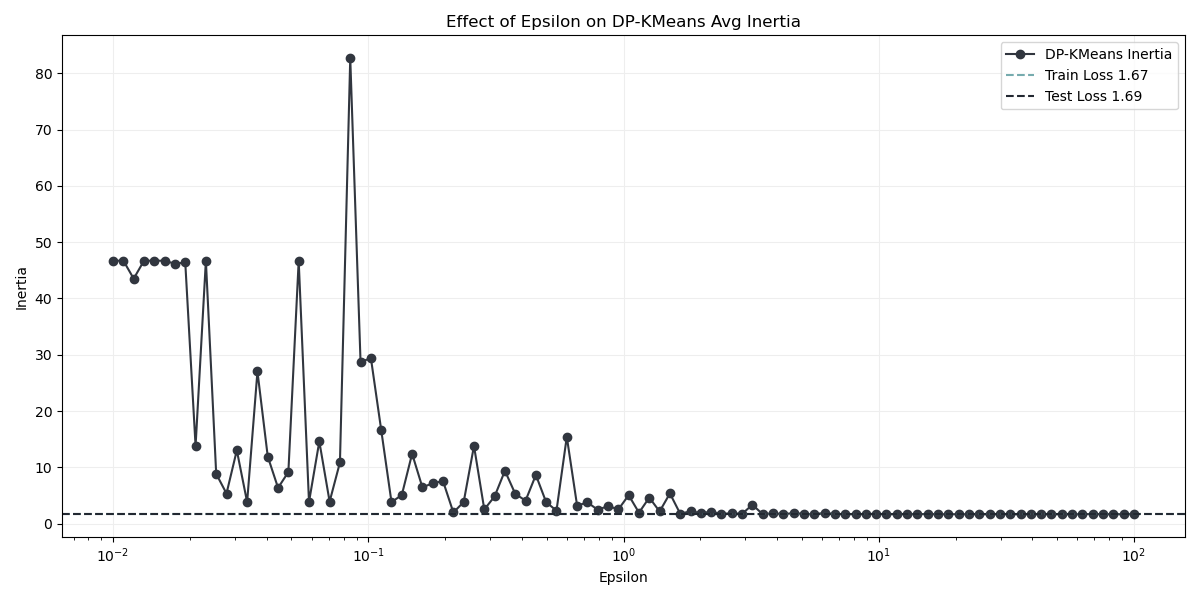
\includegraphics[width=0.6\textwidth]{figure/dpk_plot.png} % Path to the image
    \caption{Epsilon vs. Inertia compared to baseline non-private model}
    \label{fig:epsilon_inertia}
\end{figure}
\subsection{LASSO}


%%%%%%%%%%%%%%%%%%%
%%%% DISCUSSION  %%%%%%%
%%%%%%%%%%%%%%%%%%%

\section{Discussion}


\subsection{Interpretation}
Our work provides a road map for integrating differential privacy into production environments, ensuring that sensitive telemetry data can be analyzed without compromising user privacy. This is particularly relevant for industries handling large volumes of user data. 


\subsection{Limitations}



%%%%%%%%%%%%%%%%%%%
%%%% CONCLUSION %%%%%%%
%%%%%%%%%%%%%%%%%%%

\section{Conclusion}


\subsection{Summary}
Unlike previous studies that focused solely on theoretical aspects, our research demonstrates the practical feasibility of differential privacy in applied settings. Our approach offers a more accessible framework for practitioners

\subsection{Impact}


\subsection{Future Direction}



%%%%%%%%%%%%%%%%%%%%%%
%%%% CONTRIBUTIONS %%%
%%%%%%%%%%%%%%%%%%%%%%

\section{Contributions}

\subsection{Author Contributions}:
T.S. focused on task22 LASSO Regression to highlight the exploratory capabilities of private data while implementing a previously theoretical framework (Franke-Wolfe). C.L. implemented the algorithms in ... B.N. analyzed the experimental results ... T.K. analyzed the experimental results ... Y.W. supervised the research and provided guidance on the mathematical foundations. All authors contributed to writing and reviewing the manuscript.

\subsection{Task Details}

Trey Scheid
\begin{itemize}
    \item Replication of 
    \item Implementation of non-private franke-wolfe lasso regression
    \item Ethics considerations webpage
    \item [ ] Todo: Implementation of private franke-wolfe lasso regression
\end{itemize}

Tyler Kurpanek

Bradley Nathanson

Christopher Lum

Yu-Xiang Wang
\begin{itemize}
  \item Concept ideation
  \item Data Access
  \item Provided guidance on the mathematical foundations
  \item Proofing and editing all content
\end{itemize}


\subsection{Acknowledgements}

We would like to recognize the support of our instructor, Yu-Xiang Wang, for his guidance and feedback throughout the project. We would also like to thank the teaching staff Umesh Bellur and Shriniwas Kulkarni for their support and feedback. The tasks database was a foundational part of our work and was created by another student researcher: Qiyu Li. 

We also would like to thank the authors of the papers we referenced in our literature review. Their work was instrumental in our understanding of the topic and the development of our project. Our understandings of differential privacy has been built on the work of many researchers in the field such as: \_\_, \_\_, \_\_, and \_\_. Especially those which engaged in discussion with us about the field (Smith, Ulman, Guatam et al.). We are grateful for their contributions.



% COMMENT THIS BEFORE RENDERING
%\input{example_tex_section_6.tex}
% COMMENT THIS BEFORE RENDERING

%%%%%%%%%%%%%%%%%%%
%%%% REFERENCES%%%%%%%
%%%%%%%%%%%%%%%%%%%
\makereference

\bibliographystyle{style/dsc180bibstyle}


\bibliography{reference}
% To edit the contents of the ``References" section, edit \texttt{reference.bib}. Many conference websites format citations in BibTeX that you can copy into \texttt{reference.bib} directly; you can also search for the paper on Google Scholar, click ``Cite", and then click ``BibTeX" (\href{https://scholar.google.com/scholar?hl=en&as_sdt=0%2C23&q=attention+is+all+you+need&btnG=#d=gs_cit&t=1700436667623&u=%2Fscholar%3Fq%3Dinfo%3A5Gohgn6QFikJ%3Ascholar.google.com%2F%26output%3Dcite%26scirp%3D0%26hl%3Den}{here}'s an example).


%%%%%%%%%%%%%%%%%%%%%%%%%%%%%%%%%%%%%%%%%%%%%%%%%%%%%%%%
%%%% Appendix
%%%%%%%%%%%%%%%%%%%%%%%%%%%%%%%%%%%%%%%%%%%%%%%%%%%%%%%%

\clearpage
\makeappendix

\subsection{Project Proposal}


% style bad
% % !TEX TS-program = xelatex
% !BIB TS-program = bibtex
\documentclass[12pt,letterpaper]{article}
\usepackage{style/dsc180reportstyle} % import dsc180reportstyle.sty

%%%%%%%%%%%%%%%%%%%%%%%%%%%%%%%%%%%%%%%%%%%%%%%%%%%%%%%%
%%%% Title and Authors
%%%%%%%%%%%%%%%%%%%%%%%%%%%%%%%%%%%%%%%%%%%%%%%%%%%%%%%%

\title{DSC Quarter 2 Capstone Project Proposal}

\author{Bradley Nathanson \\
  {\tt bnathanson@ucsd.edu} \\\And
  Christopher Lum \\
  {\tt cslum@ucsd.edu} \\\And
  Trey Scheid \\
  {\tt tscheid@ucsd.edu} \\\And
  Tyler Kurpanek \\
  {\tt tkurpane@ucsd.edu} \\\And
  Yu-Xiang Wang \\
  {\tt yuxiangw@ucsd.edu} \\}

\begin{document}
\maketitle





\section{Proposal}
\subsection{Problem Statement}

Telemetry data is important to privatize as it encodes personally identifiable information which could be used to discover sensitive information. This data is collected from various IT devices, from satellites to personal computers. For our project, the telemetry data includes hardware and software performance metrics, monitoring, and errors. 

We will privatize 22 analysis tasks for the Intel telemetry dataset, ensuring a reasonable privacy budget (). We will implement mechanisms that balance data utility and privacy, ensuring sensitive information is protected, and allocate a reasonable privacy budget (), a parameter that governs the trade-off between accuracy and privacy.

One example of a task is to predict CPU failure. This would require a privatized logistic regression model that predicts the probability of a failure from 0-1. The model would analyze data such as CPU temperature, usage patterns, error logs, or other performance indicators. If non-privatized, this model could expose this data, as a malicious individual could do a reconstruction attack, a method to reconstruct the training data by repeatedly querying the model with various synthetic inputs. The attacker could query this model with different sets of CPU-related inputs, and, over time, the attacker could gain information such as the CPU temperature threshold for an error to occur, or whether certain system configurations have a distinct failure pattern.

\subsection{Methods}
Our methodology for privatizing the 22 telemetry analysis tasks will employ multiple privacy mechanisms, such as the exponential mechanism and the Laplace mechanism, with AutoDP serving as our core privacy accounting tool. For each analysis task, we will first evaluate the sensitivity of the computation and determine the optimal privacy mechanism to maintain utility while satisfying privacy requirements. The implementation process requires careful privacy budget allocation across multiple components of each analysis to ensure the total privacy loss remains within acceptable bounds.

The evaluation of each privatized implementation will involve a comprehensive comparison with non-private baselines to document the privacy-utility tradeoff. This includes analyzing performance metrics before and after applying privacy mechanisms, measuring accuracy degradation at various privacy budget levels, and considering computational efficiency challenges specific to telemetry data analysis. AutoDP will help quantify the privacy guarantees and guide the noise calibration process throughout implementation. 

Each privatized task will be thoroughly documented with implementation details, privacy guarantees, and performance metrics. This documentation will include privacy budget allocation strategies, noise mechanism selection rationale, and practical guidelines for future implementations. The goal is to create a comprehensive resource demonstrating how different privacy mechanisms can be effectively applied to various telemetry analysis scenarios while maintaining practical utility and ensuring strong privacy protections.


\subsection{Deliverable}
The privatized analysis tasks will be stored and shared in a public repository, (without release of source data from Intel). This is our primary contribution, to offer tools in a privatized manner. In collaboration with the accessible programs, we will publish a website that will serve to educate our peers on differential privacy. The variety of analysis tasks done in the telemetry domain can be generalized and applied to many types of data; therefore, descriptions of privacy algorithms, their motivations, and limitations can teach practitioners new methods for their own tasks. 

The Intel data as mentioned is not public (due to the customer privacy and proprietary nature). Therefore our data processing, tasks, and report will include only some metrics of performance and data quality (size, distribution, features, etc). For the information we can share, we will compare the performance of the task with that of the non-private baseline. This gives analysts a sense of the utility-privacy tradeoff in each application. 

\subsection{Impact}
By implementing differential privacy across telemetry we will create a significant impact by maintaining data confidentiality. This project will establish novel approaches to common tasks enabling hardware manufacturers to analyze system performance data while preserving strong privacy guarantees. This advances the field by demonstrating how to maintain data utility while protecting sensitive information in real-world applications. 

The research contribution includes documenting privacy-utility trade-offs and establishing guidelines for privacy budget allocation across multiple analysis tasks. Our work will demonstrate practical privacy considerations in telemetry analysis while protecting users’ participation in datasets. The methodologies developed can be adapted by other researchers working with sensitive telemetry data. 

\subsection{Success Criteria}
The success of this project is dependent on a few factors. The first two are team collaboration and schedule adherence. There are many tasks that can be privatized and there may be unique challenges for each (hence the value in sharing these!). With one-quarter complete with group work on our privatized logistic regression paper, our group is confident in our communication, task management, and problem-solving abilities. Paired with our mentor Yu-Xiang Wang, an expert in the field of differential privacy, and a seasoned professor, we are equipped to find innovative and theoretically founded methods for privatizing data tasks.

The other requirements for this project rely on data access and task availability. The Intel data is proprietary, and we have signed agreements to use the data for research, however strict access and usage terms have not been given to us yet. Previous students have worked with the contact/program at Intel successfully and we are reassured by them that we will have a usable telemetry dataset by the start of the quarter.  Similarly, there is a set of non-privatized tasks completed on this dataset by previous data scientists, their work is the foundation which we will build off of to show utility is possible even with privacy. These projects were successful implementations on the specific dataset we will have access to, this pairing therefore will continue to bear fruit as we privatize the tasks and compare baselines. 

Lastly, although we have not reviewed the dataset and tasks yet (no access), the intel program is sharing genuine telemetry information from devices with given consent as part of their program. Additionally, this HDSI-Intel partnership has been cooperating since 2020 and HDSI has used hundreds of terabytes of information. 





\end{document}

\subsubsection{Problem Statement}

Telemetry data is important to privatize as it encodes personally identifiable information which could be used to discover sensitive information. This data is collected from various IT devices, from satellites to personal computers. For our project, the telemetry data includes hardware and software performance metrics, monitoring, and errors. 

We will privatize 22 analysis tasks for the Intel telemetry dataset, ensuring a reasonable privacy budget (). We will implement mechanisms that balance data utility and privacy, ensuring sensitive information is protected, and allocate a reasonable privacy budget (), a parameter that governs the trade-off between accuracy and privacy.

One example of a task is to predict CPU failure. This would require a privatized logistic regression model that predicts the probability of a failure from 0-1. The model would analyze data such as CPU temperature, usage patterns, error logs, or other performance indicators. If non-privatized, this model could expose this data, as a malicious individual could do a reconstruction attack, a method to reconstruct the training data by repeatedly querying the model with various synthetic inputs. The attacker could query this model with different sets of CPU-related inputs, and, over time, the attacker could gain information such as the CPU temperature threshold for an error to occur, or whether certain system configurations have a distinct failure pattern.

\subsubsection{Methods}

Our methodology for privatizing the 22 telemetry analysis tasks will employ multiple privacy mechanisms, such as the exponential mechanism and the Laplace mechanism, with AutoDP serving as our core privacy accounting tool. For each analysis task, we will first evaluate the sensitivity of the computation and determine the optimal privacy mechanism to maintain utility while satisfying privacy requirements. The implementation process requires careful privacy budget allocation across multiple components of each analysis to ensure the total privacy loss remains within acceptable bounds.

The evaluation of each privatized implementation will involve a comprehensive comparison with non-private baselines to document the privacy-utility tradeoff. This includes analyzing performance metrics before and after applying privacy mechanisms, measuring accuracy degradation at various privacy budget levels, and considering computational efficiency challenges specific to telemetry data analysis. AutoDP will help quantify the privacy guarantees and guide the noise calibration process throughout implementation. 

Each privatized task will be thoroughly documented with implementation details, privacy guarantees, and performance metrics. This documentation will include privacy budget allocation strategies, noise mechanism selection rationale, and practical guidelines for future implementations. The goal is to create a comprehensive resource demonstrating how different privacy mechanisms can be effectively applied to various telemetry analysis scenarios while maintaining practical utility and ensuring strong privacy protections.


\subsubsection{Deliverable}

The privatized analysis tasks will be stored and shared in a public repository, (without release of source data from Intel). This is our primary contribution, to offer tools in a privatized manner. In collaboration with the accessible programs, we will publish a website that will serve to educate our peers on differential privacy. The variety of analysis tasks done in the telemetry domain can be generalized and applied to many types of data; therefore, descriptions of privacy algorithms, their motivations, and limitations can teach practitioners new methods for their own tasks. 

The Intel data as mentioned is not public (due to the customer privacy and proprietary nature). Therefore our data processing, tasks, and report will include only some metrics of performance and data quality (size, distribution, features, etc). For the information we can share, we will compare the performance of the task with that of the non-private baseline. This gives analysts a sense of the utility-privacy tradeoff in each application. 

\subsubsection{Impact}

By implementing differential privacy across telemetry we will create a significant impact by maintaining data confidentiality. This project will establish novel approaches to common tasks enabling hardware manufacturers to analyze system performance data while preserving strong privacy guarantees. This advances the field by demonstrating how to maintain data utility while protecting sensitive information in real-world applications. 

The research contribution includes documenting privacy-utility trade-offs and establishing guidelines for privacy budget allocation across multiple analysis tasks. Our work will demonstrate practical privacy considerations in telemetry analysis while protecting users’ participation in datasets. The methodologies developed can be adapted by other researchers working with sensitive telemetry data. 

\subsubsection{Success Criteria}

The success of this project is dependent on a few factors. The first two are team collaboration and schedule adherence. There are many tasks that can be privatized and there may be unique challenges for each (hence the value in sharing these!). With one-quarter complete with group work on our privatized logistic regression paper, our group is confident in our communication, task management, and problem-solving abilities. Paired with our mentor Yu-Xiang Wang, an expert in the field of differential privacy, and a seasoned professor, we are equipped to find innovative and theoretically founded methods for privatizing data tasks.

The other requirements for this project rely on data access and task availability. The Intel data is proprietary, and we have signed agreements to use the data for research, however strict access and usage terms have not been given to us yet. Previous students have worked with the contact/program at Intel successfully and we are reassured by them that we will have a usable telemetry dataset by the start of the quarter.  Similarly, there is a set of non-privatized tasks completed on this dataset by previous data scientists, their work is the foundation which we will build off of to show utility is possible even with privacy. These projects were successful implementations on the specific dataset we will have access to, this pairing therefore will continue to bear fruit as we privatize the tasks and compare baselines. 

Lastly, although we have not reviewed the dataset and tasks yet (no access), the intel program is sharing genuine telemetry information from devices with given consent as part of their program. Additionally, this HDSI-Intel partnership has been cooperating since 2020 and HDSI has used hundreds of terabytes of information.

\subsection{Additional Results}
example

\subsection{Training Details}
example

\subsection{Additional Figures}




\end{document}
